\section{Auswertung}
\subsection{Aufnahme der Geiger-Müller Charakteristik}
In diesem Teil des Versuches wird die Anzahl der Zerfälle in Schritten von $\Delta U= 10\,\text{V}$ gemesen (Integrationszeit $\Delta t= 60\,\text{s}$).
Die Spannungen sind von 320 bis 700V eingestellt. 
Die Intensitäten werden durch die Formel
\begin{equation}
  N = \frac{N_{60}}{60}\\
 \end{equation}
 und deren Fehler werden durch die Formel
 \begin{equation}
  \Delta N = \sqrt{N}\\
 \end{equation}
 bestimmt.
 Diese Messwerte und berechneten Werte sind in Tabelle \ref{tab:Kennlinie} aufgelistet. 
 \begin{table}[H]
  \centering
  \caption{Die Messdaten zur Geiger-Müller Kennlinie.}
  \label{tab:Kennlinie}
  \begin{tabular}{| c | c |c|c| }
  \toprule
  $U/\mathrm{V}$ & $N_{60}/\mathrm{Imp}$ & $N/\mathrm{(Imp/s)}$&$\Delta N/\mathrm{(Imp/s)}$ \\
  \midrule
  320	&9672	&161,200	& 12,696\\
330	&9689	&161,483	& 12,708\\
340	&9580	&159,667	& 12,636\\
350	&9837	&163,950	& 12,804\\
360	&9886	&164,767	& 12,836\\
370	&10041&167,350	& 12,936\\
380	&9996	&166,600	& 12,907\\
390	&9943	&165,717	& 12,873\\
400	&9995	&166,583	& 12,907\\
410	&9980	&166,333	& 12,897\\
420	&9986	&166,433	& 12,901\\
430	&9960	&166,000	& 12,884\\
440	&10219	&170,317	& 13,051\\
450	&10264	&171,067	& 13,079\\
460	&10174	&169,567	& 13,022\\
470	&10035	&167,250	& 12,933\\
480	&10350	&172,500	& 13,134\\
490	&10290	&171,500	& 13,096\\
500	&10151	&169,183	& 13,007\\
510	&10110	&168,500	& 12,981\\
520	&10255	&170,917	& 13,074\\
530	&10151	&169,183	& 13,007\\
540	&10351	&172,517	& 13,135\\
550	&10184	&169,733	& 13,028\\
560	&10137	&168,950	& 12,998\\
570	&10186	&169,767	& 13,029\\
580	&10171	&169,517	& 13,020\\
590	&10171	&169,517	& 13,020\\
600	&10253	&170,883	& 13,072\\
610	&10368	&172,800	& 13,145\\
620	&10365	&172,750	& 13,143\\
630	&10224	&170,400	& 13,054\\
640	&10338	&172,300	& 13,126\\
650	&10493	&174,883	& 13,224\\
660	&10467	&174,450	& 13,208\\
670	&10640	&177,333	& 13,317\\
680	&10939	&182,317	& 13,502\\
690	&11159	&185,983	& 13,638\\
700	&11547	&192,450	& 13,873\\
  \bottomrule
  \end{tabular}
\end{table}
\noindent
 Die Kennlinie zur Bestimmung der Charakteristik des Zählrohrs wird in Abbildung \ref{fig:Charakteristik} veranschaulicht, indem die Zählrate gegen die Spannung aufgetragen werden.

 \begin{figure}[H]
  \centering
  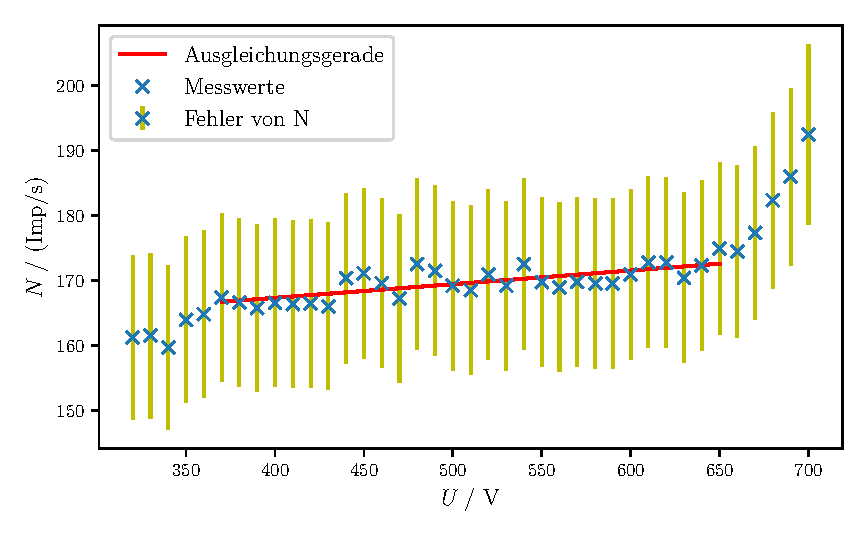
\includegraphics{Charakteristik.pdf}
  \caption{Die Kennlinie zur Bestimmung der Charakteristik des Zählrohrs.}
  \label{fig:Charakteristik}
\end{figure}
\noindent
In das Geiger-Plateau (Der Bereich wird von 370V bis 650V betrachtet) wird eine lineare Regression hinzugeführt.
Die Ausgleichsgerade besitz die Form:
\begin{equation}
 y=a\cdot t+b 
\end{equation}
mit \(y=N\), \(t=U\) .\\
Die Parameter ergeben sich zu
\begin{align*}
  a &=(0,02104 \pm 0,00369)\,\mathrm{\frac{Imp}{sV}} \\
  b &=(158,89246 \pm 1,87570)\,\mathrm{\frac{Imp}{s}} .\\
 \end{align*}
 \noindent
Der Plateauanstieg des Geiger-Muller Zahlrohres beträgt also 2,104\% 


\subsection{Bestimmung der Totzeit $T$}
\subsubsection{Zwei-Quellen-Methode}
  Als näschtes wird die Totzeit  mithilfe der zwei Quellen Methode bestimmt, in dem die $^{204} Tl-\text{Quelle}$ näher an das Geiger-Müller Zählrohr gerückt wird, um eine Totzeitkorrektur zu erhalten.
  Die Impulsraten der Quellen werden in dem Zeitintervall  $\Delta t=120 \, \text{s}$ gemessen und lauten:
  \begin{align*}
    N_{1_{120}} &=96041\, \text{Imp}\\
    N_{{1+2}_{120}} &=158479\, \text{Imp}\\
    N_{2_{120}} &=76518\, \text{Imp}.
   \end{align*} 
  Die Intensitäten werden durch die Formel (6) und deren Fehler werden durch die Formel (7) bestimmt und ergeben sich zu
  \begin{align*}
    N_1 &=(800,342\pm 28,290)\,\mathrm{Imp/s} \\
    N_{1+2} &=(1320\pm 36,341)\,\mathrm{Imp/s} \\
    N_2 &=(637,650\pm 25,252)\,\mathrm{Imp/s}.
  \end{align*} 
  Die Totzeit wird durch die Formel (5) ermittelt.
  Der Fehler für die Totzeit $T$  wird dabei über die Gau"s´sche Fehlerfortfplanzung 
  \begin{equation}
      \Delta f = \sqrt{\sum_{i=1}^N {\Bigl(\frac{\partial f}{\partial y_i}\Bigr)^2 (\Delta y_i)^2}}
  \end{equation}
 
  \begin{align*}
   \Delta T =\sqrt{\Bigl(\ \frac{N_{1+2}-N_2}{2N_1^2 N_2} \Delta N_1\Bigr)^2+\Bigl(\ \frac{N_{1+2}-N_1}{2N_1 N_2^2} \Delta N_2 \Bigr)^2+\Bigl(\ \frac{-1}{2N_1N_2} \Delta N_{1+2}\Bigr)^2}
  \end{align*}
  berechnet.
  Somit ergibt der Wert von der Totzeit $T$ zu
  \begin{align*}
    T &=(114,957 \pm 47,273)\, \mu \text{s}.
   \end{align*}


  
\subsubsection{Oszilloskop}
Die Totzeit $T$ wird in diesem Versuchteil auch mit dem Oszilloskop zu bestimmen.
Die Momentaufnahme für die Bestimmung der Totzeit $T$ ist in Abbildung \ref{fig:Oszilloskop} zu sehen.
Die Totzeit $T$ lässt sich aus dem Bild sehr ungenau ablesen und beträgt daher \( T=100\,\mu \text{s}.\)
Die  Erholungszeit  kann  aus  diesem  Bild nicht bestimmt werden.
\begin{figure}[H]
  \begin{center}
  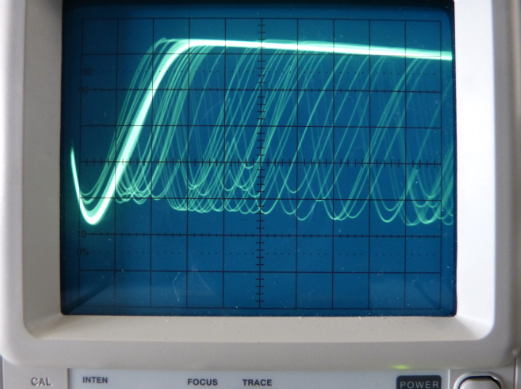
\includegraphics[width = 7cm, height= 6cm]{Oszilloskop.png}
  \caption{Momentaufnahme zur Bestimmung der Totzeit T mit dem Oszilloskop.\protect\cite{AL}}
  \label{fig:Oszilloskop}
  \end{center}
  \end{figure}

\subsection{Bestimmung des Zählrohrstroms}
Wahrend  der  Aufnahme  der  Geiger-Muller  Kennlinie (1. Teil des Versuches) wird alle 50V der Zahlrohrstrom I am Amperemeter zur Bestimmung des Zählrohrstroms abgelesen.
Die Ablesegenauigkeit am Amperemeter beträgt \(\Delta I= 0,05\,\mu \text{A}\).\\
Die Intensitäten $N$ werden durch die Formel (6) und deren Fehler $\Delta N$ werden durch die Formel (7) aus den Zählraten $N_{60}$ bestimmt.\\
Die Zahl der freigesetzten Ladungen pro eingefallenen Teilchen wird aus dem mittleren Zahlrohrstrom $I$ durch die Formel 
\begin{equation}
Z= \frac{I}{e_0 N}
\end{equation}
bestimmt.
Der Fehler von $Z$ wird durch die Gleichung (9) 
\begin{align*}
  \Delta Z =\sqrt{\Bigl(\ \frac{1}{e_0N} \Delta I\Bigr)^2+\Bigl(\ \frac{-I}{e_0 N^2} \Delta N \Bigr)^2}
 \end{align*}
gerechnet.
Diese Messwerte und berechneten Werte sind in Tabelle \ref{tab:Zählrohrstroms} aufgelistet.

\begin{table}[H]
  \centering
  \caption{Die Messdaten zur Bestimmung des Zählrohrstroms.}
  \label{tab:Zählrohrstroms}
  \begin{tabular}{| c | c |c|c|c|c|c| }
  \toprule
  $U/\mathrm{V}$ &$I/\mu \text{A} $& $N_{60}/\mathrm{Imp}$ & $N/\mathrm{(Imp/s)}$&$\Delta N/\mathrm{(Imp/s)}$ &$Z/\mathrm{(10^{10}\, Ladungen)}$&$\Delta Z/\mathrm{(10^{10}\, Ladungen)}$\\
  \midrule
  350&	0,3&	9837	&163,950	&12,804	&1,144	&0,089\\ 
  400&	0,4&	9995	&166,583	&12,907	&1,501	&0,116\\
  450&	0,7&	10264&	171,067&	13,079&	2,557&	0,196\\
  500&	0,8&	10151&	169,183&	13,007&	2,955&	0,227\\
  550&	1,0& 10184&	169,733&	13,028&	3,682&	0,283\\
  600&	1,3&	10253&	170,883&	13,072&	4,755&	0,364\\
  650&	1,4&	10493&	174,883&	13,224&	5,003&	0,378\\
  700&	1,8&	11547&	192,450&	13,873&	5,846&	0,421\\
  

  \bottomrule
  \end{tabular}
\end{table}
\noindent
Die Zahl der freigesetzten Ladungen pro eingefallenen Teilchen $Z$ wird gegen die Spannung getragen. (siehe Abbildung \ref{fig:Zaehlrohrstroms})
\begin{figure}[H]
  \centering
  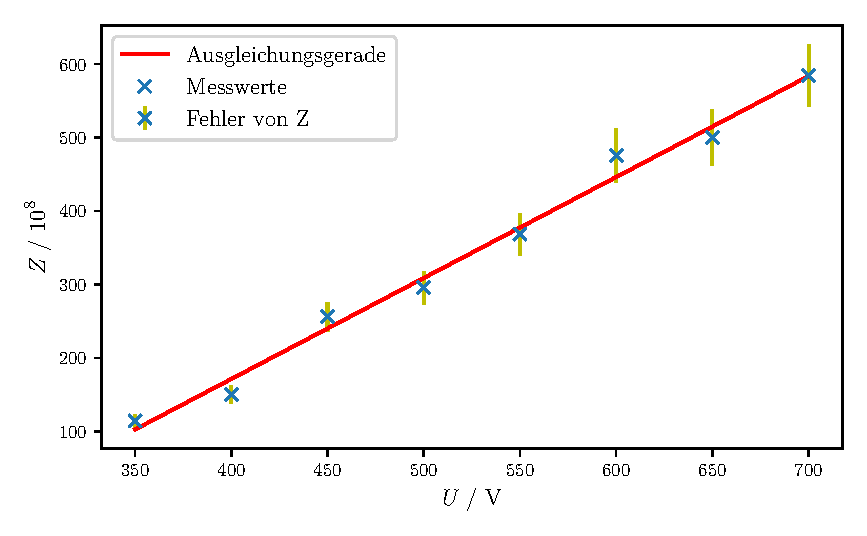
\includegraphics{Zaehlrohrstroms.pdf}
  \caption{Grafik zur Bestimmung des Zählrohrstroms.}
  \label{fig:Zaehlrohrstroms}
\end{figure}
\noindent
Die Ausgleichsgerade besitz die Form:
\begin{equation}
 y=a\cdot t+b 
\end{equation}
mit \(y=Z\), \(t=U\) .\\
Die Parameter ergeben sich zu
\begin{align*}
  a &=(1,3749 \pm 0,0587)\cdot 10^8\,\mathrm{\frac{Ladungen}{V}} \\
  b &=(-378,7815 \pm 31,5175)\cdot 10^8\,\mathrm{Ladungen} .\\
 \end{align*}



\label{sec:Auswertung}
